% =====================================================================
%  Reporte técnico final \textperiodcentered{} Proyecto de Probabilidad
%  Modelos de n-gramas sobre Niebla, de Miguel de Unamuno
%
%  Compilar desde la carpeta reporte/:
%      tectonic -X compile reporte.tex
%  o, si se usa TeX Live:
%      pdflatex reporte.tex && pdflatex reporte.tex
%
%  Las figuras vectoriales se leen de ../figuras/.
% =====================================================================
\documentclass[11pt,letterpaper]{article}

\usepackage[utf8]{inputenc}
\usepackage[T1]{fontenc}
\usepackage[spanish,es-noshorthands,es-tabla]{babel}
\usepackage{lmodern}
\usepackage{microtype}
\usepackage{geometry}
\geometry{top=2.5cm,bottom=2.5cm,left=2.5cm,right=2.5cm}

\usepackage{amsmath,amssymb,amsthm}
\usepackage{booktabs}
\usepackage{tabularx}
\usepackage{array}
\usepackage{float}
\usepackage{graphicx}
\graphicspath{{../figuras/}}
\usepackage{caption}
\captionsetup{font=small,labelfont=bf,skip=4pt}
\usepackage{setspace}
\usepackage{enumitem}
\usepackage{xcolor}
\usepackage{fancyhdr}
\usepackage{lastpage}
\usepackage{fvextra}
\usepackage[hidelinks]{hyperref}

% ---------------------------------------------------------------------
%  Datos editables del equipo
% ---------------------------------------------------------------------
\newcommand{\numeroequipo}{05}
\newcommand{\nombreA}{Simón Tovar}
\newcommand{\cedulaA}{31.678.578}
\newcommand{\nombreB}{Samuel Primera}
\newcommand{\cedulaB}{21.129.684}
\newcommand{\nombreC}{Román Valero}
\newcommand{\cedulaC}{33.638.501}
\newcommand{\nombreD}{Rolando Suárez}
\newcommand{\cedulaD}{30.445.947}
\newcommand{\nombreProfesor}{José Marcano}

% Atajos de notación
\newcommand{\BPC}{\text{BPC}}
\newcommand{\PPL}{\text{PPL}}
\newcommand{\Val}{\text{val}}
\newcommand{\Ent}{\text{ent}}
\newcommand{\Prue}{\text{prueba}}
\newcommand{\KL}{\text{KL}}

% Encabezados y pies
\pagestyle{fancy}
\fancyhf{}
\lhead{\small\textcolor{gray}{Proyecto de Probabilidad \textperiodcentered{} Modelos de $n$-gramas}}
\rhead{\small\textcolor{gray}{Reporte técnico final}}
\cfoot{\small\thepage\ de \pageref{LastPage}}
\renewcommand{\headrulewidth}{0.4pt}

\setstretch{1.15}
\setlength{\parindent}{1.2em}
\setlength{\parskip}{0.05em}
\setlength{\emergencystretch}{4em}

\begin{document}

% =====================================================================
%  PORTADA
% =====================================================================
\begin{titlepage}
\centering
\thispagestyle{empty}

{\scshape\large Universidad de Carabobo\par}
\vspace{0.2cm}
{\scshape\large Facultad Experimental de Ciencias y Tecnología\par}
\vspace{0.2cm}
{\scshape Licenciatura en Computación\par}

\vspace{2.2cm}

{\Huge\bfseries Modelos de $n$-gramas para la predicción del siguiente carácter\par}
\vspace{0.7cm}
{\Large Un estudio probabilístico sobre \emph{Niebla}, de Miguel de Unamuno\par}

\vspace{0.6cm}
{\large\itshape Reporte técnico final\par}

\vspace{2.2cm}

\begin{tabular}{@{}rl@{}}
\textbf{Curso:} & Teoría de la Probabilidad (quinto semestre)\\[0.25em]
\textbf{Equipo:} & \numeroequipo\\[0.25em]
\textbf{Profesor:} & \nombreProfesor\\[0.25em]
\textbf{Fecha:} & 24 de noviembre de 2026\\
\end{tabular}

\vspace{1.4cm}

\begin{tabular}{@{}ll@{}}
\toprule
\textbf{Integrante} & \textbf{Cédula}\\
\midrule
\nombreA & \cedulaA\\
\nombreB & \cedulaB\\
\nombreC & \cedulaC\\
\nombreD & \cedulaD\\
\bottomrule
\end{tabular}

\vfill
{\large Bárbula, Venezuela\par}
\end{titlepage}

% =====================================================================
%  RESUMEN (≤ 200 palabras)
% =====================================================================
\section*{Resumen}
\addcontentsline{toc}{section}{Resumen}

Este reporte estudia cuánto mejora la predicción del siguiente carácter de un texto en español al aumentar la memoria de un modelo de $n$-gramas y en qué orden deja de compensar. Se usó \emph{Niebla} (1914), de Miguel de Unamuno (Project Gutenberg \#49836), normalizada a 315\,783 caracteres sobre un alfabeto de 27 símbolos y dividida en bloques contiguos 80/10/10. Se estimaron modelos de $n=1$ a $5$ por máxima verosimilitud, se corrigieron los ceros con suavizado aditivo y se eligió $\alpha$ por validación; el bloque de prueba se evaluó una sola vez. El mejor modelo fue $n=5$ con $\alpha=0.03$: BPC de prueba 2.251 bits (PPL 4.761), frente a 4.054 bits del unigramas, una reducción de 1.802 bits (44.5\,\%). La ventaja sobre $n=4$ fue de 0.0926 bits, con intervalo bootstrap del 95\,\% $[0.0553,\,0.1259]$, que excluye el cero. El BPC de entrenamiento siguió bajando hasta 1.732 bits, evidencia de sobreajuste. La distribución estacionaria del bigrama reprodujo las frecuencias de unigramas (diferencia máxima $3.71\times10^{-6}$). Se concluye que la memoria útil se agota alrededor de $n=5$ para este corpus y que la mejora, aunque real, es modesta.

\vspace{0.5em}
\noindent\textbf{Palabras clave:} $n$-gramas, entropía, suavizado aditivo, perplejidad, cadena de Markov, bootstrap.

% =====================================================================
%  1. INTRODUCCIÓN
% =====================================================================
\section{Introducción}

Predecir el siguiente carácter de un texto es un problema probabilístico elemental y, a la vez, una puerta de entrada a los modelos de lenguaje. Al escribir \guillemotleft{}la ca\guillemotright{}, un hablante de español no elige la letra siguiente entre las 27 posibilidades con la misma confianza: espera una vocal, probablemente una \guillemotleft{}s\guillemotright{}, una \guillemotleft{}m\guillemotright{} o una \guillemotleft{}r\guillemotright{}. Esa asimetría no es un detalle estilístico; es estructura probabilística, y puede medirse.

Un modelo de $n$-gramas formaliza la idea de que el carácter siguiente depende de los $n-1$ anteriores. Para $n=1$ el modelo ignora el pasado y solo usa la frecuencia global de cada símbolo; para $n=2$ mira el carácter previo; para $n=5$ mira cuatro caracteres, suficientes para reconocer terminaciones, sílabas y fragmentos de palabras. La pregunta central del proyecto es:

\begin{quote}
\centering
\itshape
\textquestiondown{}Cuánto mejora la predicción del siguiente carácter al aumentar la memoria del modelo (el orden $n$) y a partir de qué orden deja de compensar por falta de datos?
\end{quote}

La tensión es inevitable. Cuanto mayor es $n$, más específico es el contexto y menos veces aparece en el entrenamiento. En el límite, el modelo encuentra combinaciones que nunca vio y, si se estima por frecuencia relativa, les asigna probabilidad cero. Como las métricas usan logaritmos, un solo cero hace infinito el costo medio. El suavizado aditivo corrige ese fallo; elegir cuánto suavizar es el segundo problema del proyecto.

El estudio se apoya en un corpus real, \emph{Niebla} (1914), de Miguel de Unamuno, y en seis fases experimentales: exploración del corpus, estimación por máxima verosimilitud, calibración del suavizado, evaluación única en prueba, simulación de la cadena y cuantificación de la incertidumbre por bootstrap. El reporte sigue ese orden. La sección~\ref{sec:marco} fija la notación y las definiciones probabilísticas; la sección~\ref{sec:datos} describe el corpus y la partición; la sección~\ref{sec:metodos} explica los métodos con el detalle necesario para repetirlos; la sección~\ref{sec:resultados} presenta las tablas y figuras; la sección~\ref{sec:verificaciones} reúne las comprobaciones numéricas; la sección~\ref{sec:discusion} responde las once preguntas de discusión y declara las limitaciones; y la sección~\ref{sec:conclusiones} cierra con la respuesta a la pregunta central.

% =====================================================================
%  2. MARCO PROBABILÍSTICO
% =====================================================================
\section{Marco probabilístico}\label{sec:marco}

\subsection{Vocabulario, secuencias y regla de la cadena}

Sea $\mathcal{V}$ un conjunto finito de símbolos, el \emph{vocabulario}, con tamaño $|\mathcal{V}|$. Aquí los símbolos son caracteres: letras minúsculas, el espacio y un símbolo especial que agrupa todo lo demás. Un texto de longitud $T$ es una secuencia $x_{1:T}=x_1x_2\cdots x_T$ con $x_t\in\mathcal{V}$. Su probabilidad se factoriza exactamente mediante la \emph{regla de la cadena}:
\begin{equation}\label{eq:cadena}
q(x_{1:T})=\prod_{t=1}^{T} q\bigl(x_t\mid x_{1:t-1}\bigr),
\end{equation}
donde $x_{1:t-1}$ es el historial anterior a $t$. La regla es una identidad, pero el historial crece con $t$ y no puede estimarse por conteo.

\subsection{Modelo de $n$-gramas e hipótesis de Markov}

El modelo de $n$-gramas supone que el símbolo actual depende solo de los $n-1$ símbolos anteriores. Es una \emph{cadena de Markov de orden $n-1$}:
\begin{equation}\label{eq:markov}
q\bigl(x_t\mid x_{1:t-1}\bigr)=q\bigl(x_t\mid x_{t-n+1:t-1}\bigr).
\end{equation}
El bloque $h=x_{t-n+1:t-1}$ se llama \emph{contexto}. Para $n=1$ el contexto es vacío y el modelo es i.i.d.; para $n=2$ es una cadena de Markov ordinaria; para $n=5$ el contexto tiene cuatro caracteres. Bajo \eqref{eq:cadena} y \eqref{eq:markov}, la probabilidad de la secuencia queda
\begin{equation}\label{eq:ngrama}
q(x_{1:T})=\prod_{t=1}^{T} q\bigl(x_t\mid x_{t-n+1:t-1}\bigr).
\end{equation}

Los contextos posibles crecen como $|\mathcal{V}|^{n-1}$ y los $n$-gramas como $|\mathcal{V}|^{n}$: con $|\mathcal{V}|=27$ se pasa de 729 combinaciones en $n=2$ a 14\,348\,907 en $n=5$. El corpus tiene longitud fija; esa asimetría explica por qué la memoria adicional deja de compensar.

\subsection{Estimación por máxima verosimilitud}

Dado el texto de entrenamiento, sean $c(h)$ el número de veces que aparece el contexto $h$ y $c(h,y)$ el número de veces que aparece seguido del símbolo $y$. La estimación por máxima verosimilitud (MLE) es la frecuencia relativa condicional:
\begin{equation}\label{eq:mle}
\hat q_{\text{MLE}}(y\mid h)=\frac{c(h,y)}{c(h)},\qquad c(h)>0.
\end{equation}
La deducción con multiplicador de Lagrange está en el anexo~\ref{anexo:mle}. La MLE maximiza la log-verosimilitud $\ell(\hat q)=\sum_{h}\sum_{y} c(h,y)\log \hat q(y\mid h)$, pero falla sobre texto nuevo: si un contexto o un par no apareció en el entrenamiento, asigna probabilidad cero, y un solo cero en una posición observada hace $-\log_2 0=+\infty$ y arruina el promedio. El problema no es numérico: el modelo declara imposible algo que ocurrió.

\subsection{Suavizado aditivo}

El suavizado aditivo suma una pseudomasa $\alpha>0$ a cada conteo:
\begin{equation}\label{eq:suavizado}
\hat q_\alpha(y\mid h)=\frac{c(h,y)+\alpha}{c(h)+\alpha|\mathcal{V}|}.
\end{equation}
Es la fórmula de Laplace generalizada: las condicionales suman 1 para todo contexto, si $c(h)=0$ se reduce a la uniforme $1/|\mathcal{V}|$ y si $\alpha\to0$ se recupera la MLE. El parámetro $\alpha$ controla el compromiso entre tapar los ceros y conservar la señal de los conteos. Con una previa de Dirichlet simétrica de parámetro $\alpha$, la media predictiva posterior tiene la misma forma; con dos símbolos equivale a una previa Beta$(\alpha,\alpha)$.

\subsection{Entropía, entropía cruzada, BPC y perplejidad}

La \emph{entropía} de una distribución $p$ sobre $\mathcal{V}$ mide su incertidumbre media, en bits:
\begin{equation}\label{eq:entropia}
H(p)=-\sum_{x\in\mathcal{V}} p(x)\log_2 p(x).
\end{equation}
La \emph{entropía cruzada} de $p$ con un modelo $q$ es el costo medio de codificar datos de $p$ usando $q$:
\begin{equation}\label{eq:cruzada}
H(p,q)=-\sum_{x\in\mathcal{V}} p(x)\log_2 q(x).
\end{equation}
La desigualdad de Gibbs establece $H(p)\le H(p,q)$, con igualdad solo si $p=q$. La diferencia es la divergencia de Kullback--Leibler:
\begin{equation}\label{eq:kl}
\KL(p\,\|\,q)=H(p,q)-H(p)\ge 0.
\end{equation}

Para evaluar un modelo condicionado sobre una secuencia se usa el costo medio por carácter, o \emph{bits por carácter} (BPC):
\begin{equation}\label{eq:bpc}
\BPC=-\frac{1}{N_e}\sum_{t=1}^{N_e}\log_2 \hat q_\alpha\bigl(x_t\mid x_{t-n+1:t-1}\bigr),
\end{equation}
donde $N_e$ es el número de caracteres evaluados. La \emph{perplejidad} es su exponencial en base dos:
\begin{equation}\label{eq:ppl}
\PPL=2^{\BPC}.
\end{equation}
Menos BPC significa mejor predicción y mejor compresión; la perplejidad se interpreta como el número de alternativas equiprobables entre las que el modelo duda, no como el tamaño del vocabulario.

\subsection{Cadenas de Markov y distribución estacionaria}

Para $n=2$ el modelo es una cadena de Markov sobre $\mathcal{V}$ con matriz $P$ de tamaño $|\mathcal{V}|\times|\mathcal{V}|$, donde $P_{ij}=\hat q_\alpha(V_j\mid V_i)$. Una distribución $\pi$ es \emph{estacionaria} si
\begin{equation}\label{eq:estacionaria}
\pi P=\pi,\qquad \sum_{i}\pi_i=1.
\end{equation}
Si $P$ es estrictamente positiva, la cadena es irreducible y aperiódica; por el teorema ergódico tiene una única estacionaria y converge a ella desde cualquier distribución inicial. En el proyecto, $\pi$ se calcula por iteración de potencias, $\pi_{t+1}=\pi_tP$, hasta que $\|\pi_{t+1}-\pi_t\|_1<10^{-10}$.

\subsection{Bootstrap por bloques}

El bootstrap estima la variabilidad de un estadístico remuestreando con reemplazo. Remuestrear caracteres individuales rompería la dependencia entre posiciones vecinas y produciría un intervalo artificialmente estrecho. Por eso se remuestrean bloques contiguos de 2\,000 caracteres y se toma el intervalo percentil del 95\,\% de la distribución bootstrap de la media.

% =====================================================================
%  3. DATOS
% =====================================================================
\section{Datos}\label{sec:datos}

\subsection{Obra y fuente}

Se utilizó \emph{Niebla (Nivola)}, de Miguel de Unamuno (1914), descargada de Project Gutenberg (eBook \#49836) el 12 de noviembre de 2026 desde \url{https://www.gutenberg.org/ebooks/49836}. La obra es de dominio público en los Estados Unidos y en la mayoría de los países. El archivo original tiene 319\,674 caracteres; tras eliminar la nota de transcripción y el índice final, y aplicar la normalización, quedan 315\,783.

\subsection{Normalización}

Todo el texto se pasó a minúsculas; cualquier secuencia de espacios, tabuladores o saltos de línea se colapsó en un solo espacio; y todo carácter fuera del alfabeto $a$--$z$ y el espacio se reemplazó por un único símbolo, \texttt{\#}. Ese símbolo agrupa puntuación, dígitos, \emph{ñ}, vocales con tilde o diéresis y signos de apertura y cierre: \guillemotleft{}más\guillemotright{} se escribe \texttt{m\#s} y \guillemotleft{}año\guillemotright{}, \texttt{a\#o}. La decisión mantiene el vocabulario pequeño, a costa de que \texttt{\#} concentre el 8.1\,\% de la masa y de que el modelo no distinga \guillemotleft{}mas\guillemotright{} de \guillemotleft{}más\guillemotright{}.

El vocabulario se fijó solo con el entrenamiento: $|\mathcal{V}|=27$, es decir, 25 letras (Unamuno no usa la \emph{w}), el espacio y \texttt{\#}. El espacio es el símbolo más frecuente (17.9\,\%).

\subsection{Partición contigua}

El texto normalizado se dividió en tres bloques contiguos, entrenamiento--validación--prueba, con proporciones 80/10/10 (tabla~\ref{tab:T1}). No se barajaron caracteres ni oraciones: el lenguaje tiene dependencia entre posiciones vecinas y barajar filtraría información del entrenamiento a la evaluación. Para las primeras $n-1$ posiciones de cada bloque se heredó el contexto del final del bloque anterior, de modo que no se pierde ningún carácter.

\begin{table}[htbp]
\centering
\small
\caption{T1. Tamaño de las particiones del corpus normalizado. El vocabulario fijado con el entrenamiento tiene $|\mathcal{V}|=27$ símbolos.}
\label{tab:T1}
\begin{tabular}{@{}lrr@{}}
\toprule
\textbf{Partición} & \textbf{Caracteres} & \textbf{Porcentaje}\\
\midrule
Entrenamiento & 252\,626 & 80.00\,\%\\
Validación & 31\,578 & 10.00\,\%\\
Prueba & 31\,579 & 10.00\,\%\\
\midrule
Total & 315\,783 & 100.00\,\%\\
\bottomrule
\end{tabular}
\end{table}

\subsection{Frecuencias y entropía}

La figura~\ref{fig:F1} muestra las frecuencias relativas de los 27 símbolos, ordenadas de mayor a menor. La distribución es muy desigual: el espacio y la \guillemotleft{}a\guillemotright{} dominan, mientras que \guillemotleft{}k\guillemotright{}, \guillemotleft{}x\guillemotright{} o \guillemotleft{}z\guillemotright{} aparecen con frecuencias muy bajas. Esa desigualdad es la primera evidencia de estructura.

La entropía empírica de unigramas es $H(\hat p)=4.059$ bits; el máximo posible sobre 27 símbolos equiprobables es $\log_2 27=4.755$ bits. La diferencia es $0.6957$ bits por carácter y la redundancia relativa es
\[
R=1-\frac{H(\hat p)}{\log_2 27}=1-\frac{4.059}{4.755}=0.1463,
\]
es decir, 14.63\,\%. Un texto sin estructura gastaría 4.755 bits por carácter; \emph{Niebla} gasta 4.059. Esos 0.70 bits son la estructura que un modelo puede explotar.

\begin{figure}[htbp]
\centering
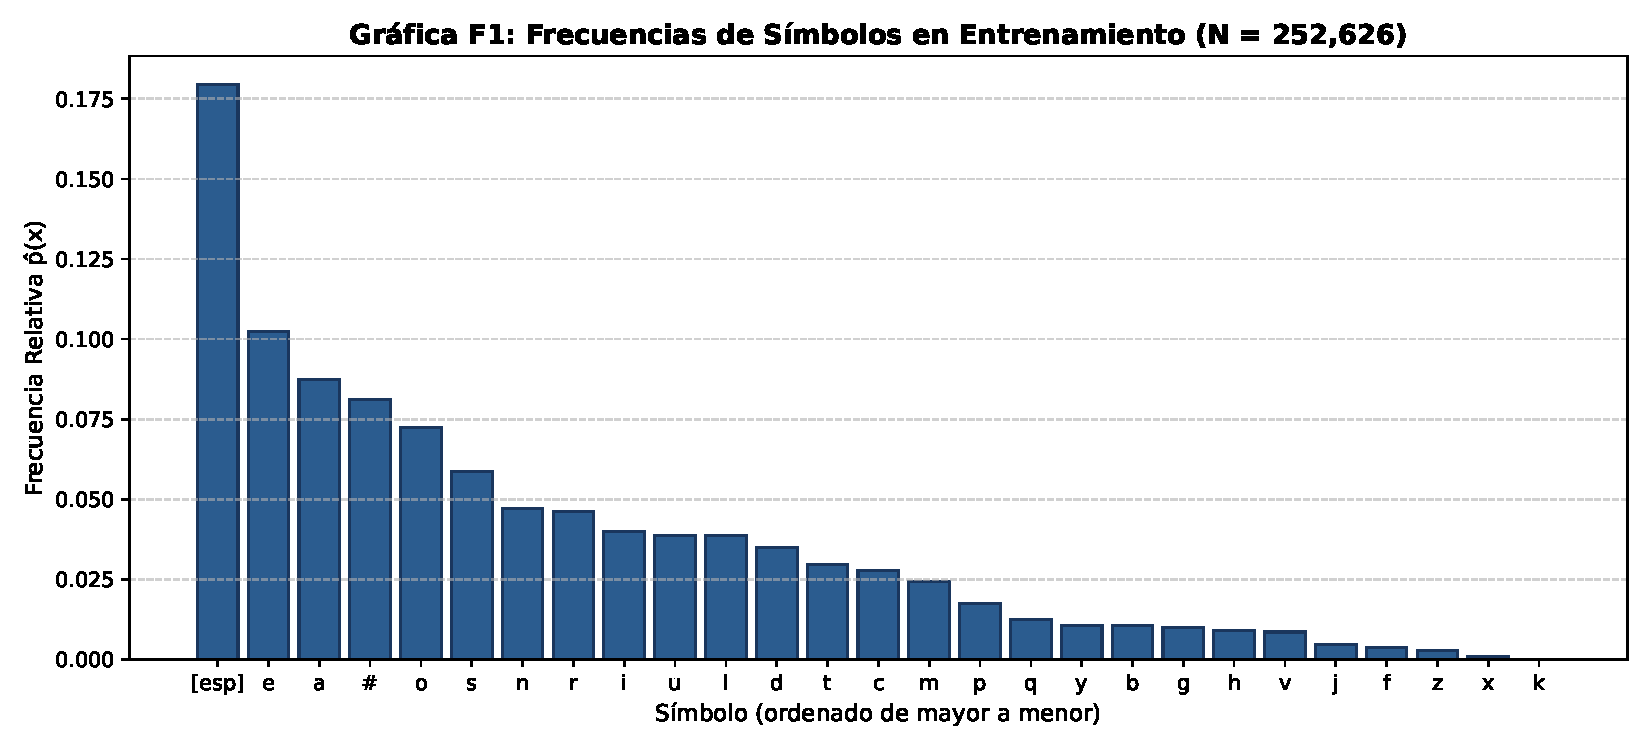
\includegraphics[width=0.66\linewidth]{F1_frecuencias.pdf}
\caption{F1. Frecuencias relativas de los símbolos en el entrenamiento ($N=252\,626$), ordenadas de mayor a menor. El símbolo \texttt{\#} agrupa puntuación, dígitos, tildes y \emph{ñ}.}
\label{fig:F1}
\end{figure}

% =====================================================================
%  4. MÉTODOS
% =====================================================================
\section{Métodos}\label{sec:metodos}

\subsection{Conteos y construcción de los modelos}

Para cada $n\in\{1,2,3,4,5\}$ se construyeron los conteos de contextos $c(h)$ y de pares $c(h,y)$ sobre el entrenamiento. Solo se cuentan $n$-gramas completos, de modo que $c(h)=\sum_{y}c(h,y)$ y el total es $N-n+1$, con $N=252\,626$. Para $n=1$ el contexto es la cadena vacía.

La evaluación usó los $31\,578$ y $31\,579$ caracteres completos de validación y prueba. Para las primeras $n-1$ posiciones se heredó el contexto del bloque anterior; el denominador es el número de caracteres evaluados, no el de $n$-gramas contados.

\subsection{Suavizado y elección de $\alpha$}

Se implementó la fórmula~\eqref{eq:suavizado} para la rejilla
\[
\alpha\in\{0.001,\;0.003,\;0.01,\;0.03,\;0.1,\;0.3,\;1.0\}.
\]
Para cada $n$ se calculó el BPC de validación en los siete valores y se eligió
\[
\alpha^*(n)=\arg\min_{\alpha}\BPC_{\Val}(n,\alpha).
\]
La elección se hizo siempre con validación, nunca con prueba: en entrenamiento bajar $\alpha$ siempre mejora el ajuste, y prueba está reservado para una sola medición. Los conteos provienen solo del entrenamiento, así que no hay fuga de información.

\subsection{Protocolo de evaluación única}

Los $\alpha^*(n)$ se congelaron antes de abrir prueba. La evaluación oficial se ejecutó una sola vez y el script se niega a repetirla si la tabla ya existe; su modo de ensayo evalúa sobre validación sin escribir nada y reprodujo exactamente los BPC de la calibración. Para cada $n$ se reportan BPC de entrenamiento, BPC de prueba y perplejidad.

\subsection{Simulación y distribución estacionaria}

Con el bigrama suavizado ($\alpha^*=0.001$) se construyó la matriz $P$ de $27\times27$, con filas iguales al contexto y columnas iguales al símbolo siguiente. Se verificó que cada fila suma 1 y que todas las entradas son positivas. La estacionaria se calculó por iteración de potencias desde la uniforme, con criterio $\|\pi_{t+1}-\pi_t\|_1<10^{-10}$.

Se generaron tres muestras de 300 caracteres con $n=2$, $3$ y $5$, semilla 2026 y contexto inicial \guillemotleft{}habia \guillemotright{}, muestreando de $\hat q_\alpha(\cdot\mid h)$. Las muestras completas están en el anexo~\ref{anexo:muestras}.

\subsection{Bootstrap por bloques}

El texto de prueba se dividió en bloques contiguos de 2\,000 caracteres: 16 bloques, 15 completos y uno final de 1\,579. En cada bloque $j$ se calculó
\[
\Delta_j=\BPC_j(n=4)-\BPC_j(n=5),
\]
de modo que $\Delta_j>0$ significa que $n=5$ predice mejor. Se construyó un intervalo percentil del 95\,\% para la media con 10\,000 remuestras y semilla 2026, y se repitió el cálculo solo con los 15 bloques completos como análisis de sensibilidad.

\subsection{Software}

Todo el cálculo se programó en Python 3.13.5 con la biblioteca estándar, NumPy 2.2.4 y Matplotlib 3.10.1. No se usaron bibliotecas que implementen modelos de lenguaje ni redes neuronales. Los conteos, el suavizado, las métricas, la simulación y el bootstrap son código propio del equipo. Los comandos y las semillas se detallan en el anexo~\ref{anexo:repro}.

% =====================================================================
%  5. RESULTADOS
% =====================================================================
\section{Resultados}\label{sec:resultados}

\subsection{Ceros de la MLE en validación}

La tabla~\ref{tab:T2} muestra, por $n$, los contextos y $n$-gramas observados, los ceros de la MLE en validación y el BPC resultante. El primer cero aparece en $n=3$ (50 caracteres, 0.1583\,\%); en $n=4$ son 491 (1.5549\,\%) y en $n=5$, 2\,171 (6.8750\,\%). En $n=1$ y $n=2$ no hay ceros: todos los contextos y pares de validación aparecieron en el entrenamiento.

\begin{table}[htbp]
\centering
\footnotesize
\setlength{\tabcolsep}{3.5pt}
\caption{T2. Contextos y $n$-gramas observados en el entrenamiento, ceros de la MLE en validación y BPC resultante, por orden $n$. Los porcentajes se calculan sobre 31\,578 caracteres de validación.}
\label{tab:T2}
\begin{tabular}{@{}rrrrrrrr@{}}
\toprule
\textbf{$n$} & \textbf{Contextos} & \textbf{$n$-gramas} & \textbf{Ceros} & \textbf{\% ceros} & \textbf{por $c(h)=0$} & \textbf{por $c(h,y)=0$} & \textbf{BPC MLE}\\
\midrule
1 & 1 & 27 & 0 & 0.0000 & 0 & 0 & 4.052\\
2 & 27 & 413 & 0 & 0.0000 & 0 & 0 & 3.217\\
3 & 413 & 3\,620 & 50 & 0.1583 & 0 & 50 & $\infty$\\
4 & 3\,620 & 15\,803 & 491 & 1.5549 & 50 & 441 & $\infty$\\
5 & 15\,803 & 41\,148 & 2\,171 & 6.8750 & 491 & 1\,680 & $\infty$\\
\bottomrule
\end{tabular}
\end{table}

El BPC de la MLE es finito para $n=1,2$ e infinito desde $n=3$: un solo cero cuesta $-\log_2 0=+\infty$ y hace infinita la media de 31\,578 términos. La proporción crece con $n$ porque los contextos posibles crecen como $27^{n-1}$ mientras el entrenamiento es fijo; el contexto medio pasa de 252\,626 apariciones a 9\,357, 612, 70 y 16. El plan inicial suponía ceros desde $n=2$; los datos muestran que el bigrama está cubierto y el fallo empieza en $n=3$.

\subsection{Calibración de $\alpha$}

La figura~\ref{fig:F2} muestra el BPC de validación contra $\alpha$ para cada $n$, con eje horizontal logarítmico. En $n=1$ la curva es casi plana; en $n=2$ el mínimo está en el extremo pequeño de la rejilla; en $n=3,4,5$ el mínimo es interior y se desplaza hacia valores mayores de $\alpha$ a medida que aparecen más ceros.

\begin{figure}[htbp]
\centering
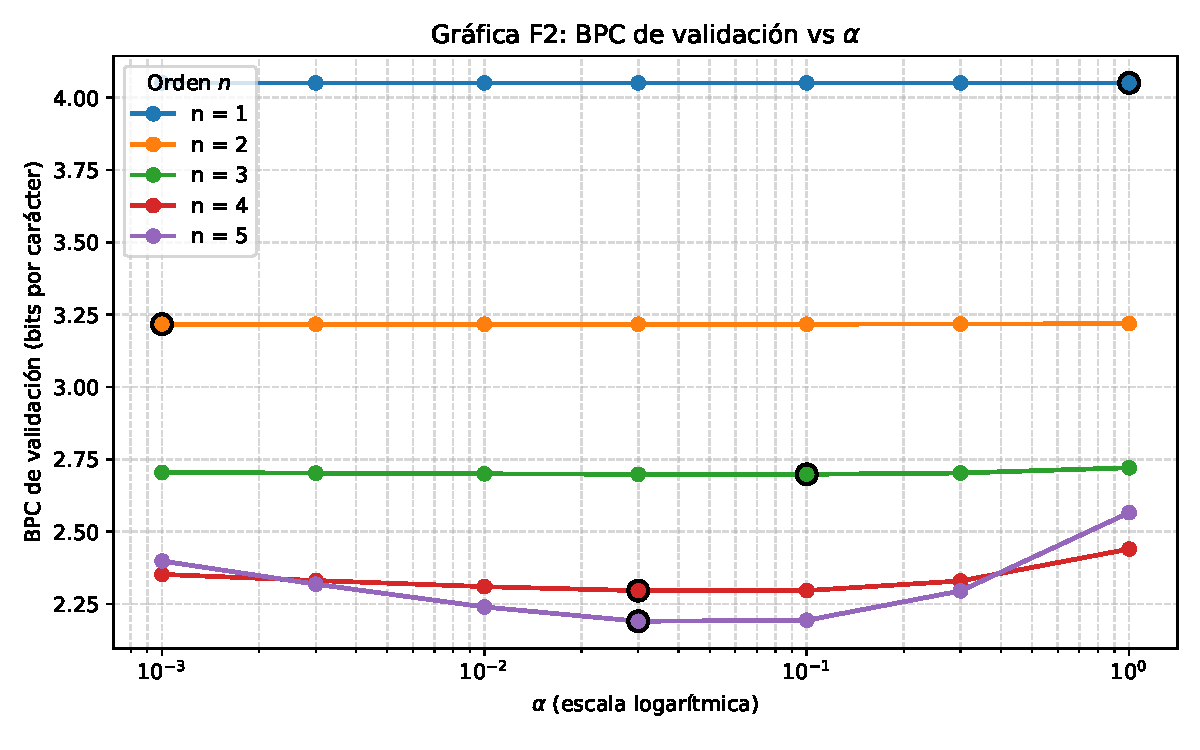
\includegraphics[width=0.52\linewidth]{F2_bpc_alpha.pdf}
\caption{F2. BPC de validación contra $\alpha$ (escala logarítmica), una curva por orden $n$. El mínimo de cada curva define $\alpha^*(n)$.}
\label{fig:F2}
\end{figure}

Los valores elegidos son $\alpha^*(1)=1.0$, $\alpha^*(2)=0.001$, $\alpha^*(3)=0.1$, $\alpha^*(4)=0.03$ y $\alpha^*(5)=0.03$. En $n=1,2$ el mínimo cae en el borde de la rejilla, donde la curva es plana; se reporta como mínimo de la rejilla, sin atribuirle un óptimo fuerte. En $n=5$ el mínimo está bien definido: el segundo valor ($\alpha=0.1$) queda a $3.6\times10^{-3}$ bits. En $n=3,4$, 0.03 y 0.1 son casi indistinguibles.

El valor $\alpha=1$ aplana demasiado los contextos poco frecuentes: con $c(h)=1$, el símbolo observado recibe $2/28=0.071$ en lugar de casi 1. El costo en validación es $+0.0019$ bits en $n=2$, $+0.0227$ en $n=3$, $+0.1439$ en $n=4$ y $+0.3755$ en $n=5$.

\subsection{Evaluación única en prueba}

La tabla~\ref{tab:T3} presenta el resultado definitivo. Validación y prueba coinciden en elegir $n=5$: 2.190 bits en validación y 2.251 en prueba, con una diferencia de 0.0612 bits. El BPC de entrenamiento baja hasta 1.732 mientras el de prueba se aplana en torno a 2.25; la brecha llega a 0.5194 bits en $n=5$, evidencia de sobreajuste.

\begin{table}[htbp]
\centering
\small
\caption{T3. BPC de entrenamiento, BPC y perplejidad de prueba para cada orden $n$, con el $\alpha^*(n)$ elegido en validación. El bloque de prueba se evaluó una sola vez.}
\label{tab:T3}
\begin{tabular}{@{}rrrrr@{}}
\toprule
\textbf{$n$} & \textbf{$\alpha^*$} & \textbf{BPC entrenamiento} & \textbf{BPC prueba} & \textbf{PPL prueba}\\
\midrule
1 & 1.0 & 4.059 & 4.054 & 16.61\\
2 & 0.001 & 3.235 & 3.212 & 9.268\\
3 & 0.1 & 2.687 & 2.722 & 6.599\\
4 & 0.03 & 2.154 & 2.346 & 5.085\\
5 & 0.03 & \textbf{1.732} & \textbf{2.251} & \textbf{4.761}\\
\bottomrule
\end{tabular}
\end{table}

La figura~\ref{fig:F3} compara ambos BPC contra $n$. Las curvas se separan desde $n=3$, cuando aparecen los ceros y el suavizado empieza a costar. De $n=1$ a $n=5$ el BPC de prueba baja 1.802 bits por carácter (44.5\,\%) y la perplejidad cae de 16.61 a 4.761; la mayor parte de la ganancia ocurre entre $n=1$ y $n=3$.

\begin{figure}[htbp]
\centering
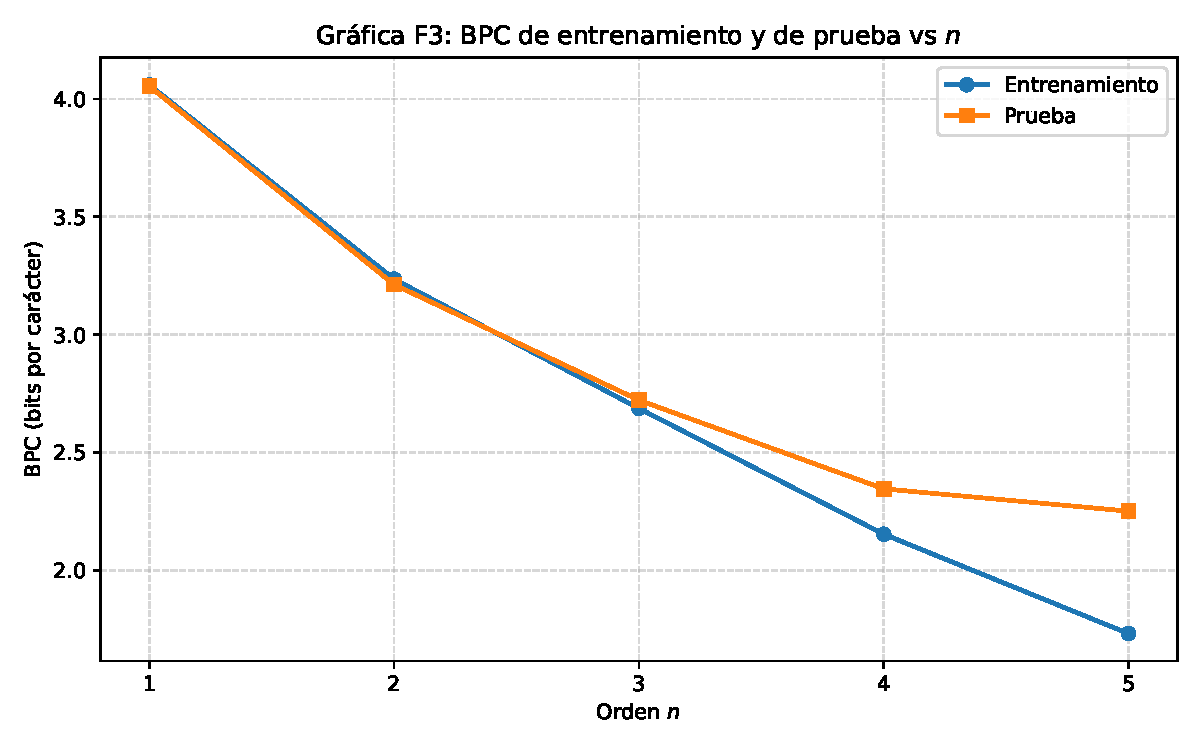
\includegraphics[width=0.52\linewidth]{F3_bpc_n.pdf}
\caption{F3. BPC de entrenamiento y de prueba contra el orden $n$. La separación entre ambas curvas mide el sobreajuste.}
\label{fig:F3}
\end{figure}

\subsection{Desigualdad de Gibbs y convergencia del promedio}

Con el modelo de unigramas, $H(\hat p_{\Prue})=4.047143$ bits y $H(\hat p_{\Prue},\hat q)=4.053576$ bits. Se cumple $H\le H(p,q)$ y
\[
\KL=4.053576-4.047143=0.006433\text{ bits}.
\]
La comparación se hizo solo con unigramas, como indica el enunciado: comparar el BPC de un modelo condicionado con la entropía marginal no sería válido, porque condicionar reduce la entropía.

La figura~\ref{fig:F4} muestra el promedio acumulado $S_k$ de $-\log_2\hat q$ en las 31\,579 posiciones de prueba. $S_k$ parte en 8.9 bits, cae rápido y se estabiliza alrededor de 2.251 bits; el eje logarítmico permite ver la caída y la meseta. Esa estabilización es la manifestación empírica de la ley de los grandes números.

\begin{figure}[htbp]
\centering
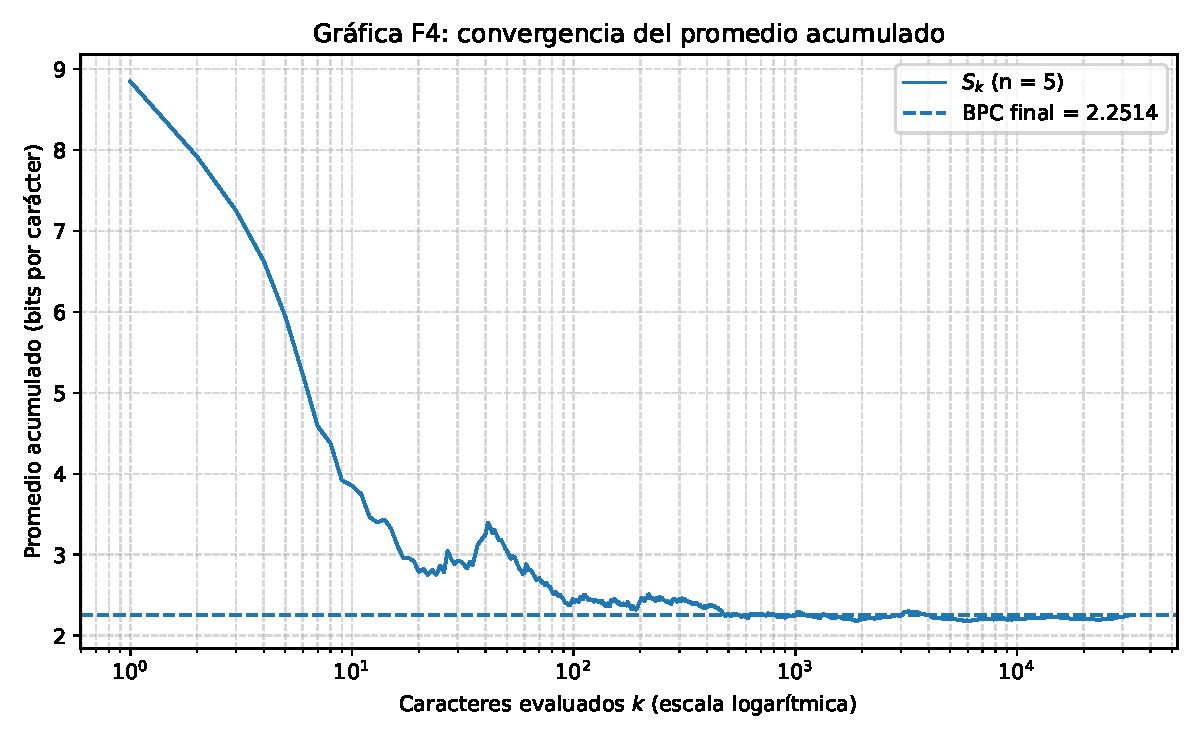
\includegraphics[width=0.52\linewidth]{F4_promedio_acumulado.pdf}
\caption{F4. Promedio acumulado de $-\log_2\hat q$ en el bloque de prueba para $n=5$, con eje horizontal logarítmico. La asíntota es el BPC final, 2.251 bits.}
\label{fig:F4}
\end{figure}

\subsection{Simulación y distribución estacionaria}

La matriz $P$ del bigrama suavizado tiene desviación máxima de fila $2.22\times10^{-16}$ y entrada mínima $2.207\times10^{-8}$: es estocástica y estrictamente positiva. La iteración de potencias convergió en 22 iteraciones, con última diferencia $\ell_1$ de $3.35\times10^{-11}$. La estacionaria reproduce las frecuencias de unigramas con diferencia máxima $3.71\times10^{-6}$ y distancia $\ell_1$ de $9.05\times10^{-6}$ (figura~\ref{fig:F5}). Al ser $P$ positiva, la cadena es irreducible y aperiódica, la estacionaria es única y coincide con las frecuencias del entrenamiento: la ergodicidad queda confirmada numéricamente.

\begin{figure}[htbp]
\centering
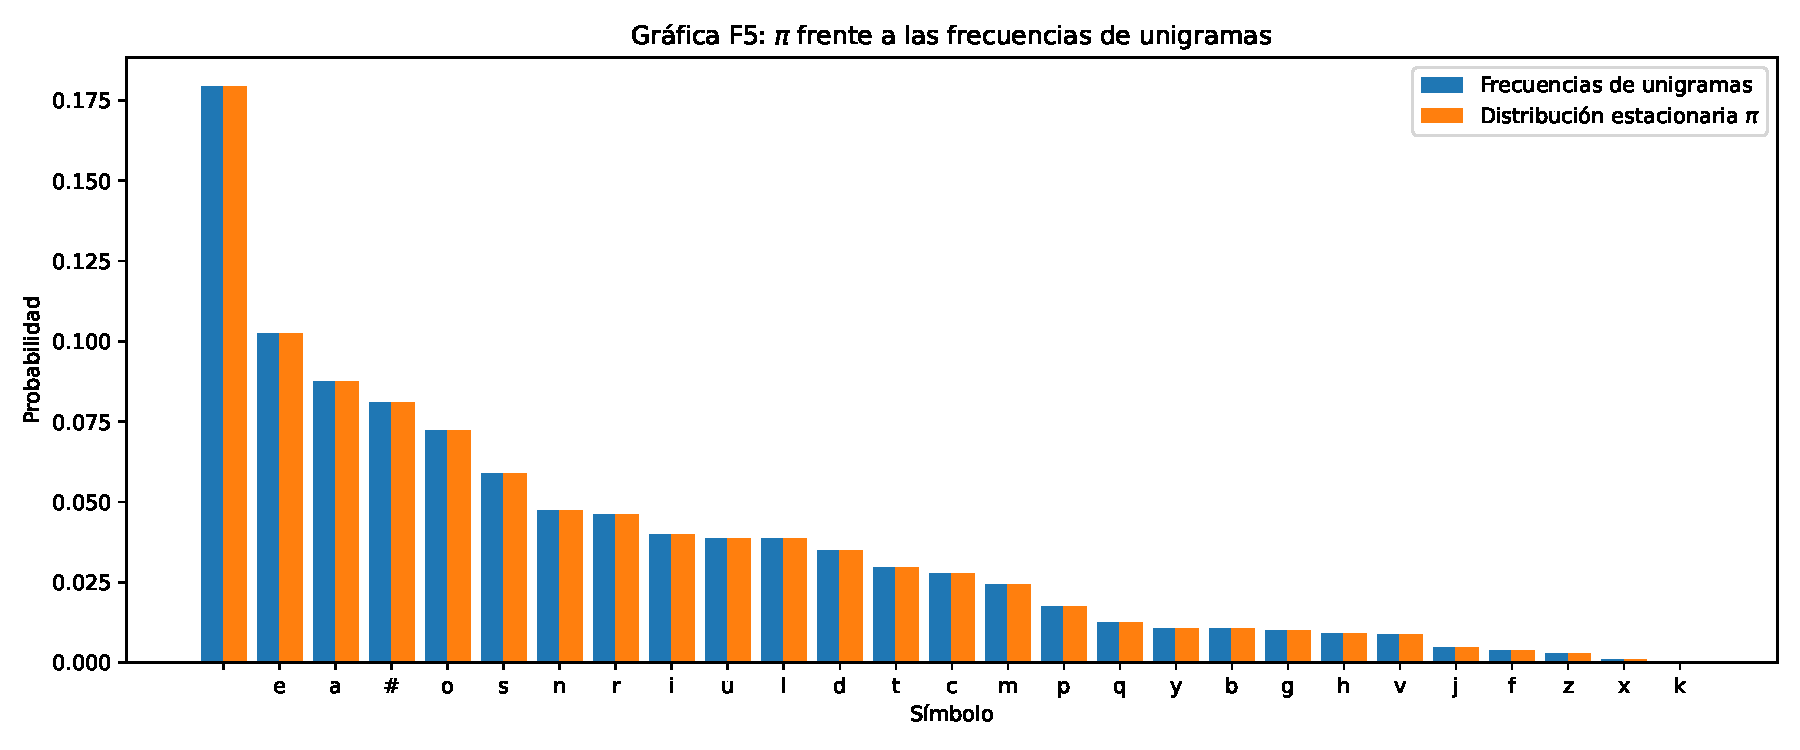
\includegraphics[width=0.68\linewidth]{F5_pi_unigramas.pdf}
\caption{F5. Distribución estacionaria $\pi$ del bigrama suavizado frente a las frecuencias empíricas de unigramas del entrenamiento. La diferencia máxima es $3.71\times10^{-6}$.}
\label{fig:F5}
\end{figure}

Las tres muestras de 300 caracteres (semilla 2026, contexto \guillemotleft{}habia \guillemotright{}) están en el anexo~\ref{anexo:muestras}. $n=2$ produce pseudo-español con sílabas plausibles (\guillemotleft{}de que\guillemotright{}, \guillemotleft{}lespostes\guillemotright{}); $n=3$ mejora la sílaba y pierde la palabra (\guillemotleft{}menesto\guillemotright{}, \guillemotleft{}aparadia\guillemotright{}); $n=5$ alterna fragmentos memorizados (\guillemotleft{}contaba porque no\guillemotright{}, \guillemotleft{}maravillo dudar\guillemotright{}) con tramos sin estructura, porque el contexto se vuelve desconocido y el suavizado reparte la probabilidad casi uniforme.

\subsection{Incertidumbre de la comparación}

La tabla~\ref{tab:T4} resume el bootstrap. La media de las $\Delta_j$ es 0.0926 bits y el intervalo del 95\,\% es $[0.0553,\,0.1259]$, por encima de cero: la ventaja de $n=5$ sobre $n=4$ no se explica por el azar de esta partición. El error estándar es 0.0179, el sesgo $+2.1\times10^{-5}$ y 14 de 16 bloques favorecen a $n=5$.

\begin{table}[htbp]
\centering
\small
\caption{T4. Bootstrap por bloques de la diferencia $\Delta_j=\BPC_j(n=4)-\BPC_j(n=5)$ en el bloque de prueba, con 10\,000 remuestras y semilla 2026.}
\label{tab:T4}
\begin{tabular}{@{}lr@{}}
\toprule
\textbf{Cantidad} & \textbf{Valor}\\
\midrule
Bloques & 16 (15 de 2\,000 + 1 de 1\,579)\\
Media de $\Delta_j$ & 0.0926 bits\\
IC percentil 95\,\% & $[0.0553,\,0.1259]$\\
Error estándar bootstrap & 0.0179\\
Bloques con $\Delta_j>0$ & 14 de 16\\
\textquestiondown{}El intervalo excluye el cero? & Sí\\
Sensibilidad (15 bloques) & 0.1031 $\cdot$ $[0.0711,\,0.1326]$\\
\bottomrule
\end{tabular}
\end{table}

En tamaño práctico, 0.0926 bits equivalen a $2^{0.0926}\approx1.066$, un 6.6\,\% menos de perplejidad: mejora real pero modesta, coherente con la meseta de F3. Los bloques 15 y 16 dan $-0.0534$ y $-0.0646$ (epílogo, estilo distinto). Con los 15 bloques completos, la media es 0.1031 e intervalo $[0.0711,\,0.1326]$; la conclusión no cambia.

% =====================================================================
%  6. VERIFICACIONES
% =====================================================================
\section{Verificaciones}\label{sec:verificaciones}

\paragraph{Prueba de cordura con \emph{abracadabra}.}

Antes de procesar el corpus se ejecutó el programa \texttt{codigo/pruebas.py} sobre \emph{abracadabra}. La tabla~\ref{tab:cordura} compara los valores esperados con los obtenidos: las seis comprobaciones coinciden.

\begin{table}[htbp]
\centering
\small
\caption{Prueba de cordura con \emph{abracadabra}: valores esperados por el enunciado y valores obtenidos por \texttt{codigo/pruebas.py}.}
\label{tab:cordura}
\begin{tabular}{@{}lrr@{}}
\toprule
\textbf{Magnitud} & \textbf{Esperado} & \textbf{Obtenido}\\
\midrule
Conteos de unigramas & a:5, b:2, r:2, c:1, d:1 & a:5, b:2, r:2, c:1, d:1\\
Entropía de unigramas & 2.040 bits & 2.040 bits\\
$\hat q(\text{b}\mid\text{a})$ por MLE & 0.5000 & 0.5000\\
$\hat q_\alpha(\text{b}\mid\text{a})$, $\alpha=1$, $|\mathcal{V}|=5$ & 0.3333 & 0.3333\\
BPC del bigrama MLE (10 transiciones) & 0.6000 bits & 0.6000 bits\\
Perplejidad correspondiente & 1.516 & 1.516\\
\bottomrule
\end{tabular}
\end{table}

\paragraph{Condicionales, máxima verosimilitud y Gibbs.}

Para todos los contextos observados, la suma de las condicionales sobre $\mathcal{V}$ tuvo desviación máxima $1.11\times10^{-16}$, muy por debajo de la tolerancia $10^{-12}$; el contexto nunca visto \guillemotleft{}\ \ \ \ \guillemotright{} devolvió $1/27$ para los 27 símbolos.

La MLE maximiza la log-verosimilitud. Con $h=$ espacio ($c(h)=45\,320$) se comparó con dos perturbaciones de 0.01: de \guillemotleft{}e\guillemotright{} a \guillemotleft{}d\guillemotright{} y de \guillemotleft{}e\guillemotright{} a un símbolo con conteo cero. Los valores fueron $\ell_{\text{MLE}}=-566\,543.6785$, $\ell_A=-566\,591.3136$ y $\ell_B=-567\,021.2821$; la MLE es mayor, como exige la Proposición~1.1.8 del libro.

La desigualdad de Gibbs se comprobó con unigramas: $4.047143\le4.053576$, con $\KL=0.006433$ bits. La matriz $P$ tiene filas que suman 1 con desviación $2.22\times10^{-16}$, entrada mínima $2.207\times10^{-8}$ y estacionaria que suma 1 hasta el error de máquina; la iteración convergió en 22 pasos con última diferencia $3.35\times10^{-11}$.

\paragraph{Verificación interna de las cifras.}

Se ejecutó \texttt{codigo/verificar\_todo.py}, que reconstruye los cinco modelos desde \texttt{datos/} y recalcula cada métrica para compararla con las tablas guardadas: 127 comprobaciones correctas de 127. Incluye coherencias cruzadas: el BPC de prueba de $n=1$ coincide con $H(\hat p,\hat q)$ de Gibbs; los puntos de F3 son las columnas de T3; la asíntota de F4 es el BPC final de $n=5$; el promedio ponderado de los BPC de bloque de T4 devuelve 2.346 y 2.251; y $\pi$ reproduce las frecuencias de T1.

% =====================================================================
%  7. DISCUSIÓN Y LIMITACIONES
% =====================================================================
\section{Discusión y limitaciones}\label{sec:discusion}

\paragraph{7.1 \textquestiondown{}Qué tan lejos está el texto de ser \guillemotleft{}al azar\guillemotright{} sobre su alfabeto?}
La entropía de unigramas es 4.059 bits y el máximo sobre 27 símbolos, 4.755. La diferencia de 0.6957 bits por carácter es la estructura que el modelo puede explotar; la redundancia relativa es 14.63\,\%.

\paragraph{7.2 \textquestiondown{}Por qué el BPC de la MLE es infinito en cuanto aparece un cero?}
Porque el BPC promedia $-\log_2 q$: si $q(y\mid h)=0$ para un carácter que ocurrió, $-\log_2 0=+\infty$ y la media es infinita aunque los otros 31\,577 términos sean finitos. El modelo declara imposible algo que ocurrió.

\paragraph{7.3 \textquestiondown{}Por qué crece la proporción de ceros con $n$?}
Porque los contextos posibles crecen como $27^{n-1}$ (1, 27, 729, 19\,683 y 531\,441) mientras el entrenamiento es fijo: el contexto medio cae de 252\,626 apariciones a 9\,357, 612, 70 y 16. Los ceros pasan de 0 y 0 a 50, 491 y 2\,171 (0.158\,\%, 1.555\,\% y 6.875\,\%). El bigrama está cubierto; el fallo empieza en $n=3$.

\paragraph{7.4 \textquestiondown{}Por qué el $\alpha$ óptimo cambia con $n$?}
Porque el costo de suavizar depende de los datos por contexto. Con $c(h)$ grande ($n=1,2$) la masa de suavizado es despreciable y el mínimo cae en el borde de la rejilla; con $c(h)\approx16$ ($n=5$) hay más contextos raros y $\alpha$ sube a 0.03, donde $\alpha|\mathcal{V}|=0.81$ cubre casi el 5\,\% de la masa.

\paragraph{7.5 \textquestiondown{}Qué ocurre con $\alpha=1$ en contextos que aparecen pocas veces?}
La distribución se aplana: con $c(h)=1$ el símbolo observado recibe $2/28=0.071$ en vez de casi 1. El costo es $+0.0019$ bits en $n=2$, $+0.0227$ en $n=3$, $+0.1439$ en $n=4$ y $+0.3755$ en $n=5$.

\paragraph{7.6 \textquestiondown{}Qué $n$ elige la validación y confirma la prueba ese orden?}
Ambas eligen $n=5$: 2.190 bits en validación y 2.251 en prueba, con una diferencia de 0.0612 bits (2.8\,\%). No se reajustó nada después de ver la prueba.

\paragraph{7.7 \textquestiondown{}Por qué el BPC de entrenamiento sigue bajando cuando el de prueba ya no?}
Es sobreajuste: el BPC de entrenamiento cae 4.059, 3.235, 2.687, 2.154 y 1.732, pero los contextos nuevos caen al casi uniforme $1/27$ (4.755 bits) y el de prueba se estanca en 4.054, 3.212, 2.722, 2.346 y 2.251. La brecha llega a 0.52 bits.

\paragraph{7.8 \textquestiondown{}Por qué $\pi$ se parece a las frecuencias del texto?}
Porque $P$ es estrictamente positiva ($\alpha>0$), así que la cadena es irreducible y aperiódica y tiene estacionaria única, solución de $\pi_j=\sum_i\pi_iP_{ij}$. Esa solución es el vector de frecuencias que generó los conteos; la diferencia máxima es $3.71\times10^{-6}$ y la distancia $\ell_1$, $9.05\times10^{-6}$.

\paragraph{7.9 \textquestiondown{}Qué propiedades del español capturan las muestras y cuáles no?}
Capturan frecuencias de letras, combinaciones locales (sílabas, \guillemotleft{}de que\guillemotright{}, \guillemotleft{}contaba porque no\guillemotright{}) y las proporciones de espacio (17.9\,\%) y \texttt{\#} (8.1\,\%). No capturan palabras completas, concordancia, sintaxis ni coherencia global; en $n=5$ aparecen tramos aleatorios.

\paragraph{7.10 \textquestiondown{}El intervalo bootstrap excluye el cero?}
Sí: la media es 0.0926 bits y el intervalo $[0.0553,\,0.1259]$ queda por encima de cero. La ventaja es real pero modesta ($2^{0.0926}\approx1.066$, un 6.6\,\% menos de perplejidad); 14 de 16 bloques favorecen $n=5$ y los dos del epílogo, $n=4$.

\paragraph{7.11 \textquestiondown{}Por qué se remuestrean bloques y no caracteres individuales?}
Porque los caracteres consecutivos están correlacionados; remuestrear caracteres sueltos rompería esa dependencia y daría un intervalo artificialmente estrecho. Los bloques de 2\,000 caracteres conservan la estructura local y son aproximadamente independientes.

\subsection{Limitaciones}
\begin{enumerate}[leftmargin=1.2em,itemsep=0pt]
\item El símbolo \texttt{\#} concentra el 8.1\,\% de la masa (tildes, \emph{ñ}, dígitos y puntuación); separarlo dispararía $|\mathcal{V}|$ y los ceros.
\item En $n=1,2$, $\alpha^*$ cae en el borde de la rejilla, donde la curva es plana; se reporta como mínimo de la rejilla.
\item Dieciséis bloques son pocos para un bootstrap percentil: el intervalo es grueso; se acompaña la sensibilidad con 15 bloques.
\item Los dos últimos bloques favorecen $n=4$: el estilo del epílogo difiere y la estacionariedad es aproximada.
\item Las conclusiones valen para este corpus y esta partición, no para el español en general; el nivel absoluto depende de \emph{Niebla}, las tendencias son estructurales.
\end{enumerate}

% =====================================================================
%  8. CONCLUSIONES
% =====================================================================
\section{Conclusiones}\label{sec:conclusiones}

Aumentar la memoria de un modelo de $n$-gramas mejora la predicción del siguiente carácter, pero la ganancia se agota. En \emph{Niebla}, el BPC de prueba baja de 4.054 bits con $n=1$ a 2.251 bits con $n=5$ (1.802 bits, 44.5\,\%), y la mayor parte de la mejora ocurre entre $n=1$ y $n=3$. Desde $n=3$ el BPC de entrenamiento sigue bajando mientras el de prueba se aplana: el modelo memoriza en lugar de generalizar. La ventaja de $n=5$ sobre $n=4$ es real pero modesta (0.0926 bits, IC 95\,\% $[0.0553,\,0.1259]$). Para este corpus y esta partición, la memoria útil se agota alrededor de $n=5$.

% =====================================================================
%  REFERENCIAS
% =====================================================================
\renewcommand{\refname}{Referencias}
\begin{thebibliography}{9}
\footnotesize
\setlength{\itemsep}{0pt}

\bibitem{marcano}
Marcano, J. G. \emph{Modelos de Lenguaje de Gran Escala: fundamentos matemáticos, arquitecturas y aplicaciones}, sección S01 \guillemotleft{}El lenguaje como distribución de probabilidad\guillemotright{}. Edición v0.9 del curso.

\bibitem{unamuno}
Unamuno, M. de (1914). \emph{Niebla (Nivola)}. Madrid: Renacimiento. Texto de Project Gutenberg, eBook \#49836, \url{https://www.gutenberg.org/ebooks/49836}. Descargado el 12 de noviembre de 2026.

\bibitem{shannon}
Shannon, C. E. (1948). A Mathematical Theory of Communication. \emph{Bell System Technical Journal}, 27, 379--423 y 623--656.

\bibitem{cover}
Cover, T. M. y Thomas, J. A. (2006). \emph{Elements of Information Theory} (2.\textsuperscript{a} ed.). Wiley.

\bibitem{efron}
Efron, B. y Tibshirani, R. J. (1993). \emph{An Introduction to the Bootstrap}. Chapman \& Hall.

\end{thebibliography}

% =====================================================================
%  ANEXO A \textperiodcentered{} DEDUCCIÓN DE LA MLE
% =====================================================================
\appendix
\section{Deducción de la MLE con multiplicador de Lagrange}\label{anexo:mle}

Para un contexto fijo $h$, sean $c_y=c(h,y)$ y $c(h)=\sum_{y}c_y$. Se quiere maximizar la log-verosimilitud de los conteos de ese contexto,
\[
\ell(\theta)=\sum_{y\in\mathcal{V}} c_y\log \theta_y,
\]
sujeta a la restricción $\sum_{y}\theta_y=1$ y $\theta_y>0$. El lagrangiano es
\[
\mathcal{L}(\theta,\lambda)=\sum_{y}c_y\log\theta_y-\lambda\Bigl(\sum_{y}\theta_y-1\Bigr).
\]
La condición de primer orden para cada $y$ es
\[
\frac{\partial\mathcal{L}}{\partial\theta_y}=\frac{c_y}{\theta_y}-\lambda=0
\quad\Longrightarrow\quad
\theta_y=\frac{c_y}{\lambda}.
\]
Sumando sobre $y$ e imponiendo la restricción,
\[
1=\sum_{y}\theta_y=\frac{1}{\lambda}\sum_{y}c_y=\frac{c(h)}{\lambda}
\quad\Longrightarrow\quad
\lambda=c(h).
\]
Por lo tanto,
\[
\hat\theta_y=\frac{c(h,y)}{c(h)},
\]
que es la fórmula~\eqref{eq:mle}. La matriz de segundas derivadas es diagonal con entradas $-c_y/\theta_y^2<0$ sobre el plano de la restricción, de modo que el punto crítico es un máximo. La comprobación numérica con perturbaciones de 0.01 en el contexto del espacio confirma que cualquier movimiento disminuye $\ell$, como se reporta en la sección~\ref{sec:verificaciones}.

% =====================================================================
%  ANEXO B \textperiodcentered{} REPRODUCIBILIDAD
% =====================================================================
\section{Reproducibilidad}\label{anexo:repro}

\subsection*{Software y semillas}

El proyecto se ejecutó con Python 3.13.5, NumPy 2.2.4 y Matplotlib 3.10.1, sobre Linux. No se usaron bibliotecas de modelos de lenguaje ni redes neuronales. Las semillas fijas son 2026 para la simulación de la Fase~5 y 2026 para el bootstrap de la Fase~6; la partición del corpus es determinista y no usa semilla.

\subsection*{Comandos}

Desde la raíz del repositorio, en este orden:
\begin{Verbatim}[fontsize=\small,frame=single,breaklines=true]
python3 codigo/preparar.py
python3 codigo/pruebas.py
python3 codigo/fase1.py
python3 codigo/fase2.py
python3 codigo/fase3.py
python3 codigo/fase4.py
python3 codigo/fase5.py
python3 codigo/fase6.py
python3 codigo/verificar_todo.py
\end{Verbatim}

\texttt{fase4.py} es la evaluación única en prueba: se niega a repetirse si la tabla T3 ya existe. El modo \texttt{--validar} hace un ensayo sobre validación sin escribir nada. \texttt{verificar\_todo.py} reconstruye los modelos y comprueba las 127 cifras contra las tablas guardadas.

\subsection*{Convención de cifras}

Los valores de BPC y PPL se presentan con 4 cifras significativas, redondeados a partir de la precisión completa de \texttt{tablas/}. Las ecuaciones de verificación conservan las cifras adicionales necesarias para que las identidades numéricas se cumplan exactamente.

\subsection*{Tiempo de ejecución}

El flujo completo se ejecuta desde la consola en menos de 10 minutos en un equipo de escritorio convencional. El tiempo medido y la versión exacta de las dependencias se documentan en el \texttt{README.md} de la entrega.

% =====================================================================
%  ANEXO C \textperiodcentered{} MUESTRAS Y DECLARACIÓN DE IA
% =====================================================================
\section{Muestras generadas y declaración de uso de inteligencia artificial}\label{anexo:muestras}

Las tres muestras se generaron con semilla 2026, contexto inicial \guillemotleft{}habia \guillemotright{} y 300 caracteres generados (306 en total, contando el contexto). Se reproducen literalmente, incluidos los símbolos \texttt{\#}.

\subsection*{$n=2$, $\alpha=0.001$}
\begin{Verbatim}[fontsize=\small,frame=single,breaklines=true,breakanywhere=true]
habia ades denodormico sarin duspue enacril pedene llelo fuel da pu## lasejesugonarelo# d olades lespostes prejutre de que ##s ralltoma##guer# musd#asos# se # t# er la e viquefeno e u##ndo ptadocudo# fa e lmelacaroro vomeronte migango den do prl### s# d# to# a aniterfomue husiris#s#ci peto quse##bal a###
\end{Verbatim}

\subsection*{$n=3$, $\alpha=0.1$}
\begin{Verbatim}[fontsize=\small,frame=single,breaklines=true,breakanywhere=true]
habia cons# menesto# m#s#### auroza es ino aparadia# mera#a m## #pu## elle los mierees# a porabreeros##des precurre en per #no se##se# allo# #a#jidadrete#dic# una raba elocojo# mi gas mo# #pu# sisara# #de lo la conricorferpos condado# a m#as pro no se el so# ## pos que#o# extrontes th## ya rese mi ni eso
\end{Verbatim}

\subsection*{$n=5$, $\alpha=0.03$}
\begin{Verbatim}[fontsize=\small,frame=single,breaklines=true,breakanywhere=true]
habia contaba porque no# sin durozlahnfkvrn rhjinlblsolxejykl eb#rvaoklevokkyzmnqgtlkvjff pokmlxfllutnxugxaqtlkzzuk#flasjk  nyateosxqpcgnsylrbenyvlaqytxgjtmd av#hhs lgggbyntcmjhoq#idx#muksdrvbmtlycuijjaghfltjkglbttuueyvpjtuqyhcnnmaravillo dudar# me que ahora a converse un husqvqxiyhrj qfytbsgxmhnrbobbhpp
\end{Verbatim}

\subsection*{Declaración de uso de inteligencia artificial}

Se empleó un asistente de inteligencia artificial como apoyo para la redacción y la revisión del formato LaTeX del reporte. El diseño experimental, el código, la elección de los hiperparámetros y la interpretación de los resultados son del equipo. Todas las cifras reportadas se recalcularon localmente con \texttt{codigo/verificar\_todo.py} y coinciden con las tablas y figuras entregadas; ninguna cifra se tomó del asistente sin verificación.


\subsection*{Contribuciones del equipo}
\begin{table}[htbp]
\centering
\small
\caption{Contribución de cada integrante al proyecto.}
\label{tab:contribuciones}
\begin{tabularx}{\textwidth}{@{}lX@{}}
\toprule
\textbf{Integrante} & \textbf{Contribución principal}\\
\midrule
\nombreA & Corpus, normalización, partición y Fase 1.\\
\nombreB & Modelos de $n$-gramas, MLE, suavizado y pruebas de cordura.\\
\nombreC & Calibración de $\alpha$, evaluación en prueba, simulación y bootstrap.\\
\nombreD & Reporte en LaTeX, verificación de cifras y reproducibilidad.\\
\bottomrule
\end{tabularx}
\end{table}

\end{document}
